\section{Background On Looplets}
Finch represents iteration patterns using Looplets, a language that decomposes
datastructure iterators hierarchically. 
%
Looplets represent the control-flow
structures needed to iterate over any given datastructure, or multiple
datastructures simultaneously. 
%
In particular, looplets are good at lifting code
to the highest loop level that it's needed and subdividing iteration
hierarchically in coordinate space.
%
Because looplets are compiled with
progressive lowering, structure-specific mathematical optimizations such as
integrals, multiply by zero, etc. can be implemented using simple compiler
passes like term rewriting and constant propagation during the intermediate
lowering stages. \cite{ahrens_looplets_2023}

In this work, we partially simplify the presentation of Looplets to focus on the
semantics, rather than precise implementation. Since Finch is designed to be
embedded into another language\saman{not clear}, we allow for several of the looplets to utilize
functions that modify the state of that language. It is assumed that if a
looplet introduces a variable to be used in a child looplet, the child looplet
will not modify that variable.\saman{No context yet to understand this. Need to introduce what looplets are (Fig 2)!}

\begin{figure}[ht]
    \scriptsize
    \begin{minipage}[c]{0.6\linewidth}
        $\finchlookup(seek, body)$: The Lookup Looplet represents a
        randomly accessible region of an iterator. The body of the lookup is
        understood to have one less dimension than the lookup itself, as we have
        already ``looked up'' that index in the tensor by the time we reach the
        body. \texttt{seek(i)} is a function that updates state to the given
        index.
    \end{minipage}%
    \begin{minipage}[c]{0.4\linewidth}
        \centering
        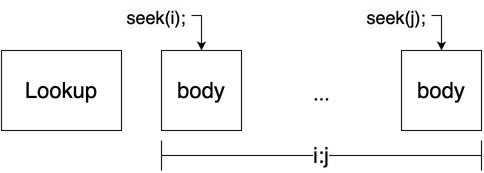
\includegraphics[scale=0.25]{Looplets-lookup.png}
    \end{minipage}

    \begin{minipage}[c]{0.6\linewidth}
        $\finchrun(body)$: The Run Looplet represents a constant
        region of an iterator. The body of the run is understood to have one
        less dimension than the lookup itself, as all of the bodies are
        identical.
    \end{minipage}%
    \begin{minipage}[c]{0.4\linewidth}
        \centering
        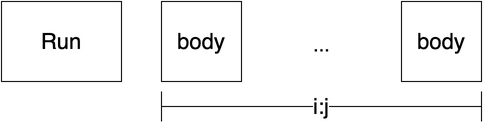
\includegraphics[scale=0.25]{Looplets-run.png}
    \end{minipage}

    \begin{minipage}[c]{0.6\linewidth}
        $\finchphase(c:d, body)$: The Phase Looplet represents a
        restriction of the range on which a loop should execute, and allows us
        to succinctly express the ranges on which children of compound looplets
        are defined.
    \end{minipage}%
    \begin{minipage}[c]{0.4\linewidth}
        \centering
        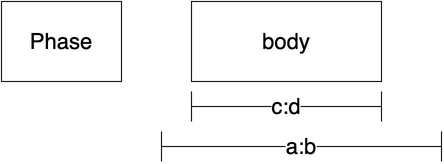
\includegraphics[scale=0.25]{Looplets-phase.png}
    \end{minipage}
    \begin{minipage}[c]{0.6\linewidth}
        $\finchswitch(cond, head, tail)$: The Switch Looplet allows
        us to specialize the body of a looplet based on a condition, evaluated
        in the embedding context. If the condition is true, we use `head`,
        otherwise we use `tail`. Switch has a high lowering priority so we can
        see what's inside of it and lower that appropriately. This also lifts
        the condition as high as possible into the loop nest. The condition is
        assumed to evaluate to a boolean.
    \end{minipage}%
    \begin{minipage}[c]{0.4\linewidth}
        \centering
        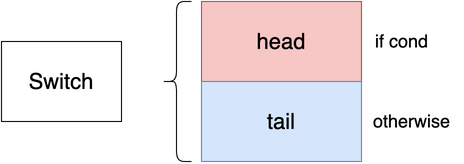
\includegraphics[scale=0.25]{Looplets-switch.png}
    \end{minipage}
    \begin{minipage}[c]{0.6\linewidth}
        $\finchthunk(preamble, body, epilogue)$: The Thunk Looplet
        allows us to cache certain computations in the state under which the
        body will execute. This is useful for computing and caching the results
        of expensive computations.
    \end{minipage}%
    \begin{minipage}[c]{0.4\linewidth}
        \centering
        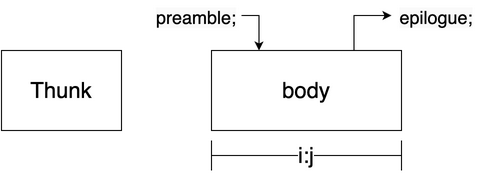
\includegraphics[scale=0.25]{Looplets-thunk.png}
    \end{minipage}

    \begin{minipage}[c]{0.6\linewidth}
        $\finchsequence(head, tail)$: The Sequence looplet represents the
        concatenation of two looplets. Both arguments must be phase looplets, and
        are assumed to be nonoverlapping, covering, and in order.
    \end{minipage}%
    \begin{minipage}[c]{0.4\linewidth}
        \centering
        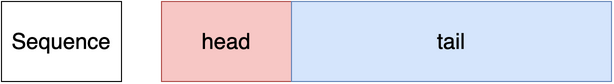
\includegraphics[scale=0.25]{Looplets-sequence.png}
    \end{minipage}

    \begin{minipage}[c]{0.6\linewidth}
        $\finchspike(body, tail)$ The Spike Looplet represents a run
        followed by a single value. In this paper, Spike will be considered a
        shorthand for $\finchsequence(\finchphase(i:j-1, \finchrun(body)),
        \finchphase(j:j, \finchrun(tail)))$.  In the Finch compiler, spikes are
        handled with special care, since they are an opportunity to align the
        final run to the end of the root loop extent, without using any special
        bounds inference.
    \end{minipage}%
    \begin{minipage}[c]{0.4\linewidth}
        \centering
        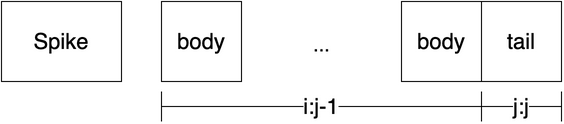
\includegraphics[scale=0.25]{Looplets-spike.png}
    \end{minipage}

    \begin{minipage}[c]{0.6\linewidth}
        $\finchstepper([seek], next, body)$ The stepper looplet
        represents a variable number of looplets, concatenated. Since our
        looplets may be skipped over due to conditions or various rewrites, the
        $seek$ function allows us to fast-forward the state to the start of the
        root loop extent when it comes time to lower the stepper. The $next$
        function advances the state to the next iteration of the stepper. 
    \end{minipage}%
    \begin{minipage}[c]{0.4\linewidth}
        \centering
        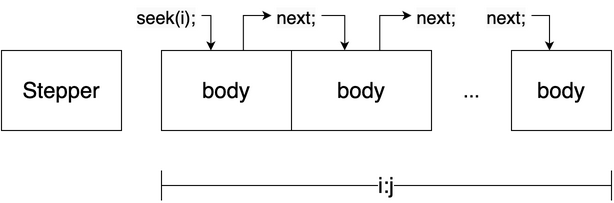
\includegraphics[scale=0.25]{Looplets-stepper.png}
    \end{minipage}
    \vspace{-8pt}
    \caption{The looplet language, as understood in a correct execution of a Finch program.}

\end{figure}